% Preamble
% ---
\documentclass{article}

% Packages
% ---
\usepackage{amsmath} % Advanced math typesetting
\usepackage[utf8]{inputenc} % Unicode support (Umlauts etc.)
\usepackage[ngerman]{babel} % Change hyphenation rules
\usepackage{hyperref} % Add a link to your document
\usepackage{graphicx} % Add pictures to your document
\usepackage{listings} % Source code formatting and highlighting
\usepackage{booktabs}

\renewcommand{\figurename}{Figure}
%\usepackage[labelsep=endash]{caption}

\usepackage{xcolor}
\lstset { %
    language=C++,
    backgroundcolor=\color{black!5}, % set backgroundcolor
    basicstyle=\footnotesize,% basic font setting
}



\title{%
	MA226 : Monte-Carlo Simulation\\
	 Brownian Motion\\
	 \large Assignment 10}

\date{6-04-2017}

\author{%
	Turkhade Hrushikesh Pramod\\
	150123044	}	

\begin{document}

	\maketitle
	\pagenumbering{gobble}
	
	\newpage
	\pagenumbering{arabic}
	
	\section{Problem 1}
	\paragraph{}
		We have to generate 10 sample paths from standard brownian motion.
	\paragraph{}
	\[W(t_{i+1}) = W(t_i)+\sqrt{t_{i+1}-t_i}.Z_{i+1}\]
		
	\subsection{Source code of the solution}
		\lstinputlisting[language=R,firstline=1]{code/que1.R}
		
	\subsection{Observation}

	
Expected Value of w(2) :  -0.06535669 \\
Expected Value of w(5) :  1.021281\\

	\clearpage

		\subsection{Plots}
	
		\paragraph{}
		In the following plots, each color represents unique brownian path.		
		
			\begin{figure}[!ht]
  			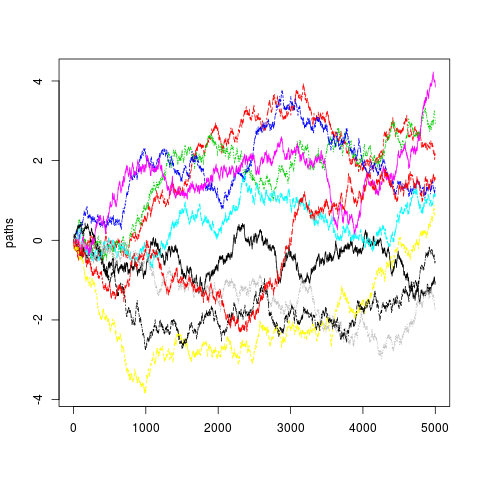
\includegraphics[width=\linewidth]{pic/que1_single.png}
 			 \caption{Paths for standard Brownian Motion.}
  			\label{fig:hist1_1}
		\end{figure}
		
		\clearpage
	
		
	
	\section{Problem 2}
	\paragraph{}
		We have to generate 10 sample paths from brownian motion with $mean=0.06$ and $sigma=0.3$.
		
	\paragraph{}
	\[X(t_{i+1}) = X(t_i)+\mu(t_{i+1}-t_{i})+\sigma\sqrt{t_{i+1}-t_i}.Z_{i+1}\]
		
	\subsection{Source code of the solution}
		\lstinputlisting[language=R,firstline=1]{code/que2.R}
		
	
		\subsection{Observation}

	
Expected Value of w(2) :  4.818397 \\
Expected Value of w(5) :  4.986213	\\

\clearpage
	
		\subsection{Plots}
	
		\paragraph{}
		In the following plots, each color represents unique brownian path.
		
			\begin{figure}[!ht]
  			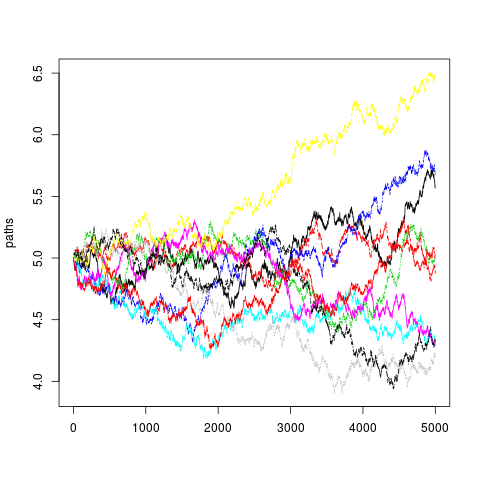
\includegraphics[width=\linewidth]{pic/que2.png}
 			 \caption{Paths for standard Brownian Motion.}
  			\label{fig:hist1_1}
		\end{figure}
		
		\clearpage
		
	\section{Problem 3}
	\paragraph{}
		We have to generate 10 sample paths from brownian motion with $mu(t)=0.0325-0.05t$ and $sigma(t)=0.012 + 0.0138t+0.00125{t^2}$.
	
	\paragraph{}
	\[Y(t_{i+1}) = Y(t_i)+\mu(t_i)(t_{i+1}-t_{i})+\sigma(t_i)\sqrt{t_{i+1}-t_i}.Z_{i+1}\]
		
	\subsection{Source code of the solution}
		\lstinputlisting[language=R,firstline=1]{code/que3.R}
	
	\subsection{Observation}

	
Expected Value of w(2) :  4.97063 \\
Expected Value of w(5) :  4.586572\\
	
		\pagebreak
		\subsection{Plots}
	
		\paragraph{}
		In the following plots, each color represents unique brownian path.
		
			\begin{figure}[!ht]
  			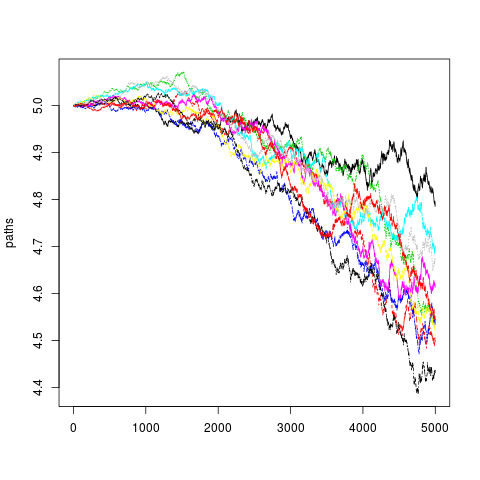
\includegraphics[width=\linewidth]{pic/que3.png}
 			 \caption{Paths for given Brownian Motion.}
  			\label{fig:hist1_1}
		\end{figure}
		
		\clearpage

\end{document}